\documentclass[a4paper,12pt]{report}

% Global commands
\newcommand{\reportTitle}{
    \textcolor{black}{The Design of a PocketQube Satellite Communication System}
}

\newcommand{\reportSubtitle}{
    \textcolor{black}{}
}

\newcommand{\nameInitial}{
    \textcolor{black}{G. Allen}
}
\newcommand{\nameFull}{
    \textcolor{black}{Gary Allen}
}
\newcommand{\stNumber}{
    \textcolor{black}{23905093}
}
\newcommand{\myDate}{\textcolor{black}{\today}
}

% Page layout
\usepackage[left=2.2cm,right=2.2cm,top=2.2cm,bottom=2.2cm]{geometry}

% Figures
\usepackage[margin=\the\parindent,small,bf,sf]{caption}
\usepackage{graphicx}
\usepackage{pdfpages}
\setlength{\abovecaptionskip}{7.5pt}  % spacing above and below captions
\newcommand*{\WaterMark}[2][0.2\paperwidth]{\AddToShipoutPicture*{\AtTextCenter{\parbox[c]{0pt}{\makebox[0pt][c]{\includegraphics[width=#1]{#2}}}}}}
\usepackage{subcaption}

% Font and text
\usepackage[english]{babel}
\usepackage{microtype}
\usepackage{setspace}
\usepackage{lmodern}
\newcommand{\myemph}[1]{{\sffamily\bfseries#1}}
\sloppy
\onehalfspacing
\usepackage{siunitx}
\usepackage{lipsum}

% Headings
\usepackage[raggedright,sf,bf]{titlesec}
\titleformat{\chapter}[display] {\normalfont\bfseries}{}{0pt}{\Huge}
\titleformat{\chapter}[hang]{\Huge\bfseries}{\thechapter{. }}{0pt}{\Huge\bfseries}

% Table of contents
\makeatletter
\let\originall@chapter\l@chapter
\def\l@chapter#1#2{\originall@chapter{{\sffamily #1}}{#2}}
\makeatother
\let \savenumberline \numberline
\def \numberline#1{\savenumberline{#1.}}

% Mathematics
\usepackage[cmex10]{amsmath}
\usepackage{amssymb}
\usepackage{cancel}
\DeclareMathOperator*{\argmax}{arg\,max}
\newcommand{\T}{^\textrm{T}}
\newcommand{\tr}{\textrm{tr}}
\renewcommand{\vec}[1]{\boldsymbol{\mathbf{#1}}}
\newcommand{\defeq}{\triangleq}

% Tables
\usepackage{booktabs}
\usepackage{tabularx}
\usepackage{multirow}
\newcommand{\mytable}{
    \centering
    \small
    \renewcommand{\arraystretch}{1.2}
    }
\renewcommand{\tabularxcolumn}[1]{m{#1}}
\newcolumntype{C}{>{\centering\arraybackslash}X}
\newcolumntype{L}{>{\raggedright\arraybackslash}X}

% Header and footer
\usepackage{fancyhdr}
\pagestyle{fancy}
\fancyhf{}
\renewcommand{\sectionmark}[1]{\markright{\normalsize \thesection.\ #1}}
\fancyhead[C]{\nouppercase{\textit{\rightmark}}}
\fancyhead[RO]{\thepage}
\fancyfoot{}
\setlength\headheight{14.5pt}
\renewcommand{\headrulewidth}{0pt}
\fancypagestyle{plain}{\fancyhead{}
                       \renewcommand{\headrulewidth}{0pt}
                       \fancyfoot[C]{\thepage}}

% Pseudo-code
\usepackage{algorithm}  % should go before \usepackage{hyperref}

% Table of contents and hyperlinks
\usepackage{hyperref}
\hypersetup{colorlinks=true,linktoc=all,citecolor=black,linkcolor=black}
\usepackage[nottoc]{tocbibind}

% Pseudo-code
\usepackage{algpseudocode}  % should go after \usepackage{hyperref}
\renewcommand{\thealgorithm}{\arabic{chapter}.\arabic{algorithm}} 
\captionsetup[algorithm]{labelfont={bf,sf},font=small,labelsep=colon}

% Bibliography
\usepackage{cite}  % automatically reorder inline citations
\bibliographystyle{IEEEtran}

% Fix titlesec issue
\usepackage{etoolbox}
\makeatletter
\patchcmd{\ttlh@hang}{\parindent\z@}{\parindent\z@\leavevmode}{}{}
\patchcmd{\ttlh@hang}{\noindent}{}{}{}
\makeatother
 \usepackage[normalem]{ulem}


% Document 
\begin{document}

% Front matter
\graphicspath{{./figures/}}
\pagenumbering{Alph}

\begin{titlepage}
\begin{center}


\includegraphics[width=8cm]{SU_logo_RGB_without_slogan.pdf}

\vfill

{\sffamily \bfseries \huge \reportTitle \par}

{\sffamily \bfseries \Large \reportSubtitle \par}

\vfill

{\large {\Large \nameFull} \\ \stNumber \par}

\vfill

\vfill

\vfill

\vfill

{\Large \myDate}
\end{center}
\end{titlepage}

%\chapter*{Declaration}
\newpage
\thispagestyle{plain}
\addcontentsline{toc}{chapter}{Declaration}
\makeatletter\@mkboth{}{Declaration}\makeatother

\centerline{
\includegraphics[width=8cm]{USlogo-top}}
\vspace*{-10pt}

\section*{\centering Plagiaatverklaring / \textit{Plagiarism Declaration}}

\vspace*{5pt}

\begin{enumerate}
    \item Plagiaat is die oorneem en gebruik van die idees, materiaal en ander intellektuele eiendom van ander persone asof dit jou eie werk is.\\
    \textit{Plagiarism is the use of ideas, material and other intellectual property of another's work
        and to present it as my own.}
    
    \item Ek erken dat die pleeg van plagiaat 'n strafbare oortreding is aangesien dit 'n vorm van diefstal is.\\
    \textit{I agree that plagiarism is a punishable offence because it constitutes theft.}
    
    \item Ek verstaan ook dat direkte vertalings plagiaat is. \\
    \textit{I also understand that direct translations are plagiarism.}
    
    \item Dienooreenkomstig is alle aanhalings en bydraes vanuit enige bron (ingesluit die internet) volledig verwys (erken). Ek erken dat die woordelikse aanhaal van teks sonder aanhalingstekens (selfs al word die bron volledig erken) plagiaat is. \\
    \textit{Accordingly all quotations and contributions from any source whatsoever (including the internet) have been cited fully. I understand that the reproduction of text without quotation marks (even when the source is cited) is plagiarism}
    
    \item Ek verklaar dat die werk in hierdie skryfstuk vervat, behalwe waar anders aangedui, my eie oorspronklike werk is en dat ek dit nie vantevore in die geheel of gedeeltelik ingehandig het vir bepunting in hierdie module/werkstuk of 'n ander module/werkstuk~nie. \\
    \textit{I declare that the work contained in this assignment, except where otherwise stated, is my original work and that I have not previously (in its entirety or in part) submitted it for grading in this module/assignment or another module/assignment.}
\end{enumerate}

\vfill

\noindent \begin{tabularx}{1.0\linewidth}{|L|L|}
    \hline
    \vspace{1cm} {Studentenommer / \textit{Student number}} & \vspace{1cm} {Handtekening / \textit{Signature}} \\
    \hline
    \vspace{1cm} {Voorletters en van / \textit{Initials and surname}} & \vspace{1cm} {Datum / \textit{Date}} \\
    \hline
\end{tabularx}

\vspace{15pt}

% The old declaration

%I, the undersigned, hereby declare that the work contained in this report is my own original work unless otherwise stated.
%
%% Afrikaans:
%% Hiermee verklaar ek, die ondergetekende, dat die werk in hierdie verslag vervat my eie oorspronklike werk is, tensy anders vermeld.
%
%\vspace{2.5cm}
%
%\begin{table}[h]
%\begin{tabular}{@{}p{2.5cm}p{5cm}}
%    Signature: & \dotfill \\
%    & \multicolumn{1}{c}{Obi-Wan Kenobi} \\
%    ~\vspace{1cm} \\
%    Date: & \dotfill \\
%\end{tabular}
%\end{table}
%
%\vfill
%
%\begin{center}
%    Copyright \textcopyright\ 2099 Stellenbosch University \\
%    All rights reserved
%\end{center}


\pagenumbering{roman}
\tableofcontents
\listoffigures
\listoftables
\chapter*{Nomenclature\markboth{}{Nomenclature }}
\addcontentsline{toc}{chapter}{Nomenclature}

% \vspace*{-3mm}
\subsubsection*{Variables and functions}
\begingroup
\renewcommand{\arraystretch}{1.2}
\renewcommand{\tabularxcolumn}[1]{p{#1}}
\begin{tabularx}{\textwidth}{@{}p{2.5cm}L}
    $V$     & Voltage \\
    $I$     & Current \\
    $R$     & Resistance \\
\end{tabularx}
\endgroup


%\newpage
\subsubsection*{Acronyms and abbreviations}

\begingroup
\renewcommand{\arraystretch}{1.2}
\begin{tabular}{@{}p{2.5cm} l}
    GS       & GroundStation \\
    PQ       & PocketQube \\
\end{tabular}
\endgroup

\chapter*{Abstract}
\addcontentsline{toc}{chapter}{Abstract}
\makeatletter\@mkboth{}{Abstract}\makeatother

\subsubsection*{English}

This report documents the design and implementation of a wireless communication system for a miniaturised satellite called a \textit{PocketQube}. The PocketQube standard is a set of specifications which aim to make it easier for people to design small satellite modules that can easily integrate with each other. The standard is relatively new, however, and few designs have been published for a full PocketQube communication system that includes a ground station.

The design in this project includes both a tracking ground station, as well as a PocketQube module. The LoRa-based ground station was designed to mechanically track the satellite system using a pre-defined GPS path, as well as using satellite-received GPS data. The system was then implemented, and the communication link was tested up to 100 km line-of-sight and found to be reliable at a baud rate of 9600 bps. This report documents the design choices made and constraints faced, analyses the measured results of the system, and suggests improvements for future projects.

\selectlanguage{english}
\newpage
\pagenumbering{arabic}

% Contents
\chapter{Introduction}

This project aims to design and implement a wireless communication system for a miniaturised satellite called a PocketQube (PQ). The PocketQube standard was created to define physical and electronic requirements for so-called "nano satellites". The goal of this is to allow for easy integration of various sub-modules into one physical enclosure. One common use-case of these satellites is to collect sensory information from the atmosphere. These can either be placed into orbit, are attached to a \textit{high-altitude balloons} (e.g. a large, helium balloon). In this project, such a balloon will been provided by the department, and a communication system for this satellite balloon will be designed.

This project consists of the design of three sub-systems. The communication system to be designed will involve both a tracking ground station (GS), as well as a PQ 'unit'. The general idea is that the GS will mechanically track the PQ while it communicates with it, enabling realtime data transmission and telemetry. An existing two-axis antenna mount has been provided for the GS, which a newly-designed PCB will be placed into. The GS will mechanically the balloon, allowing bi-directional wireless communication. The PQ unit should conform to the PQ standard and fit inside a provided housing. The third sub-system is the integration of a proprietary Radiosonde (atmospheric telemetry device) into the newly-designed communication system.

Literature will be consulted in order to investigate the various design approaches and decisions. Since the project focuses on system design and integration, a number of components and sub-modules will ultimately be combined to form the final system. Different electronic components and their specifications will be compared based on gathered project requirements. This will require trade-offs to be made, since the system design is limited in time, cost, form-factor and several other factors. This report documents the trade-offs and decisions made, with the goal of being of use to future designers of similar systems.
\chapter{Problem Definition}

\section{Requirements}

The requirements for this project are defined by analysing general existing balloon-satellite systems, as well as taking into account the planned launch that this specific PQ will be used in. In these systems, the high-altitude balloons can drift to a height of around 30 km \cite{weatherWeatherBalloons}.
\chapter{Background}

\graphicspath{{./figures}}

\section{PocketQube}

The PocketQube standard is a fairly new set of protocols and specifications defining a modularized nano-satellite system. The term \textit{modularized} in this context refers to the ability for different "modules" or PocketQube units, each with their own set functionality, to be connected to a common \textit{backplane} and integrate seamlessly. \textit{Integration} here refers to both the mechanical spacing of each module, as well as the electronic communication between the modules.

\begin{figure}[!htb]
    \centering
    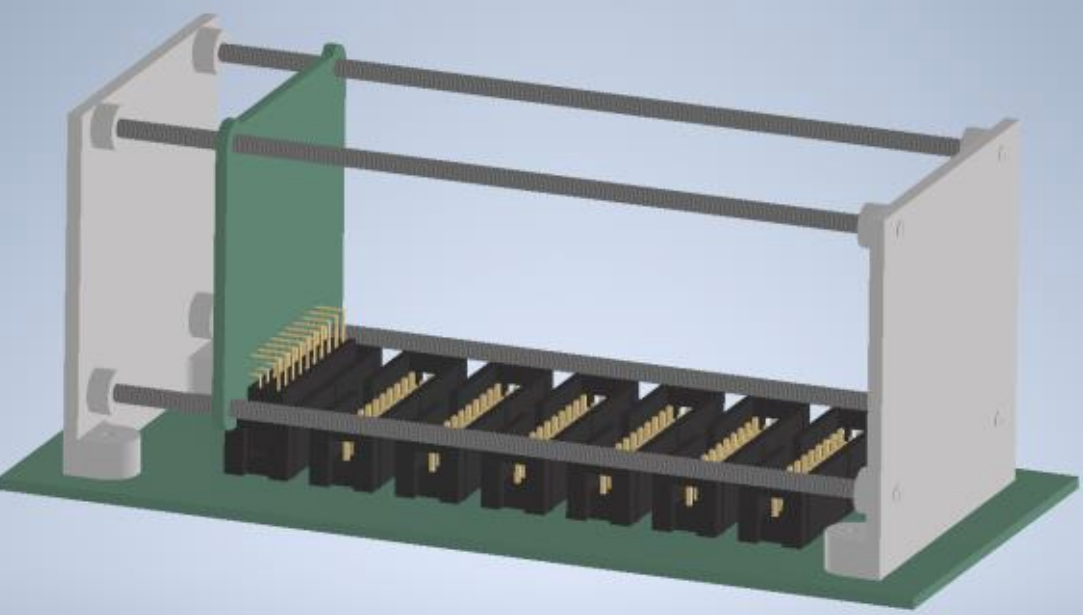
\includegraphics[width=0.6\textwidth]{pq_enclosure}
    \caption{A PQSU Enclosure \cite{standard-pqsu}}
    \label{fig:pq_enclosure}
\end{figure}

As an example, a PocketQube enclosure could contain three units: a communication module, a sensor pack, and a battery system. These modules can then be connected onto the backplane via headers, and placed inside a single enclosure, such as that in Figure \ref{fig:pq_enclosure}. This "nano-satellite" can then be "launched" through any means.
\chapter{Conclusion}

The conclusion

% Bibliography
\nocite{*}
\bibliography{references}

% End matter
\appendix
% Appendix A
\chapter{Appendix A}
\subfile{planning/planning.tex}

% Appendix B
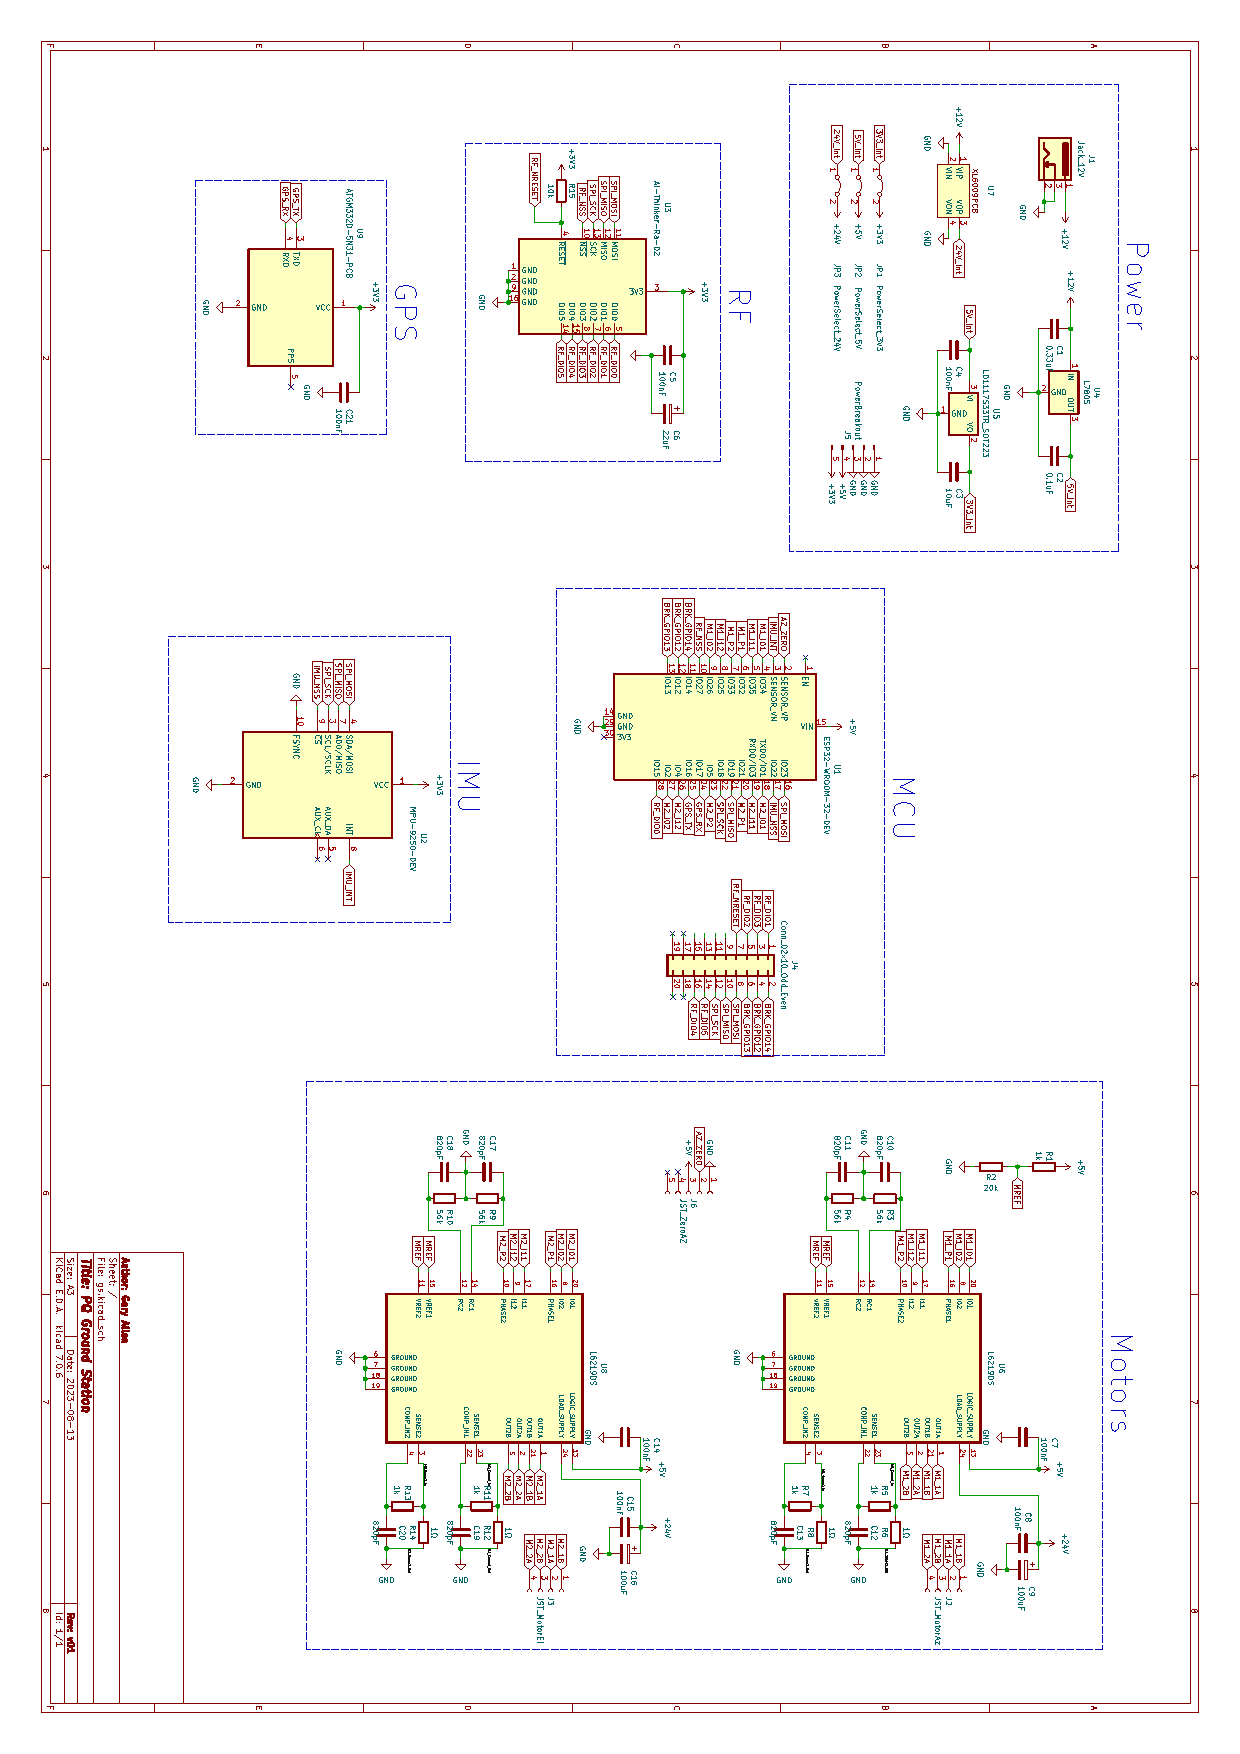
\includepdf[scale=0.55,pages=1,pagecommand=\chapter{Appendix B}\label{sec:appendix_gs_schematics}]{gs_schematic}

% Appendix C
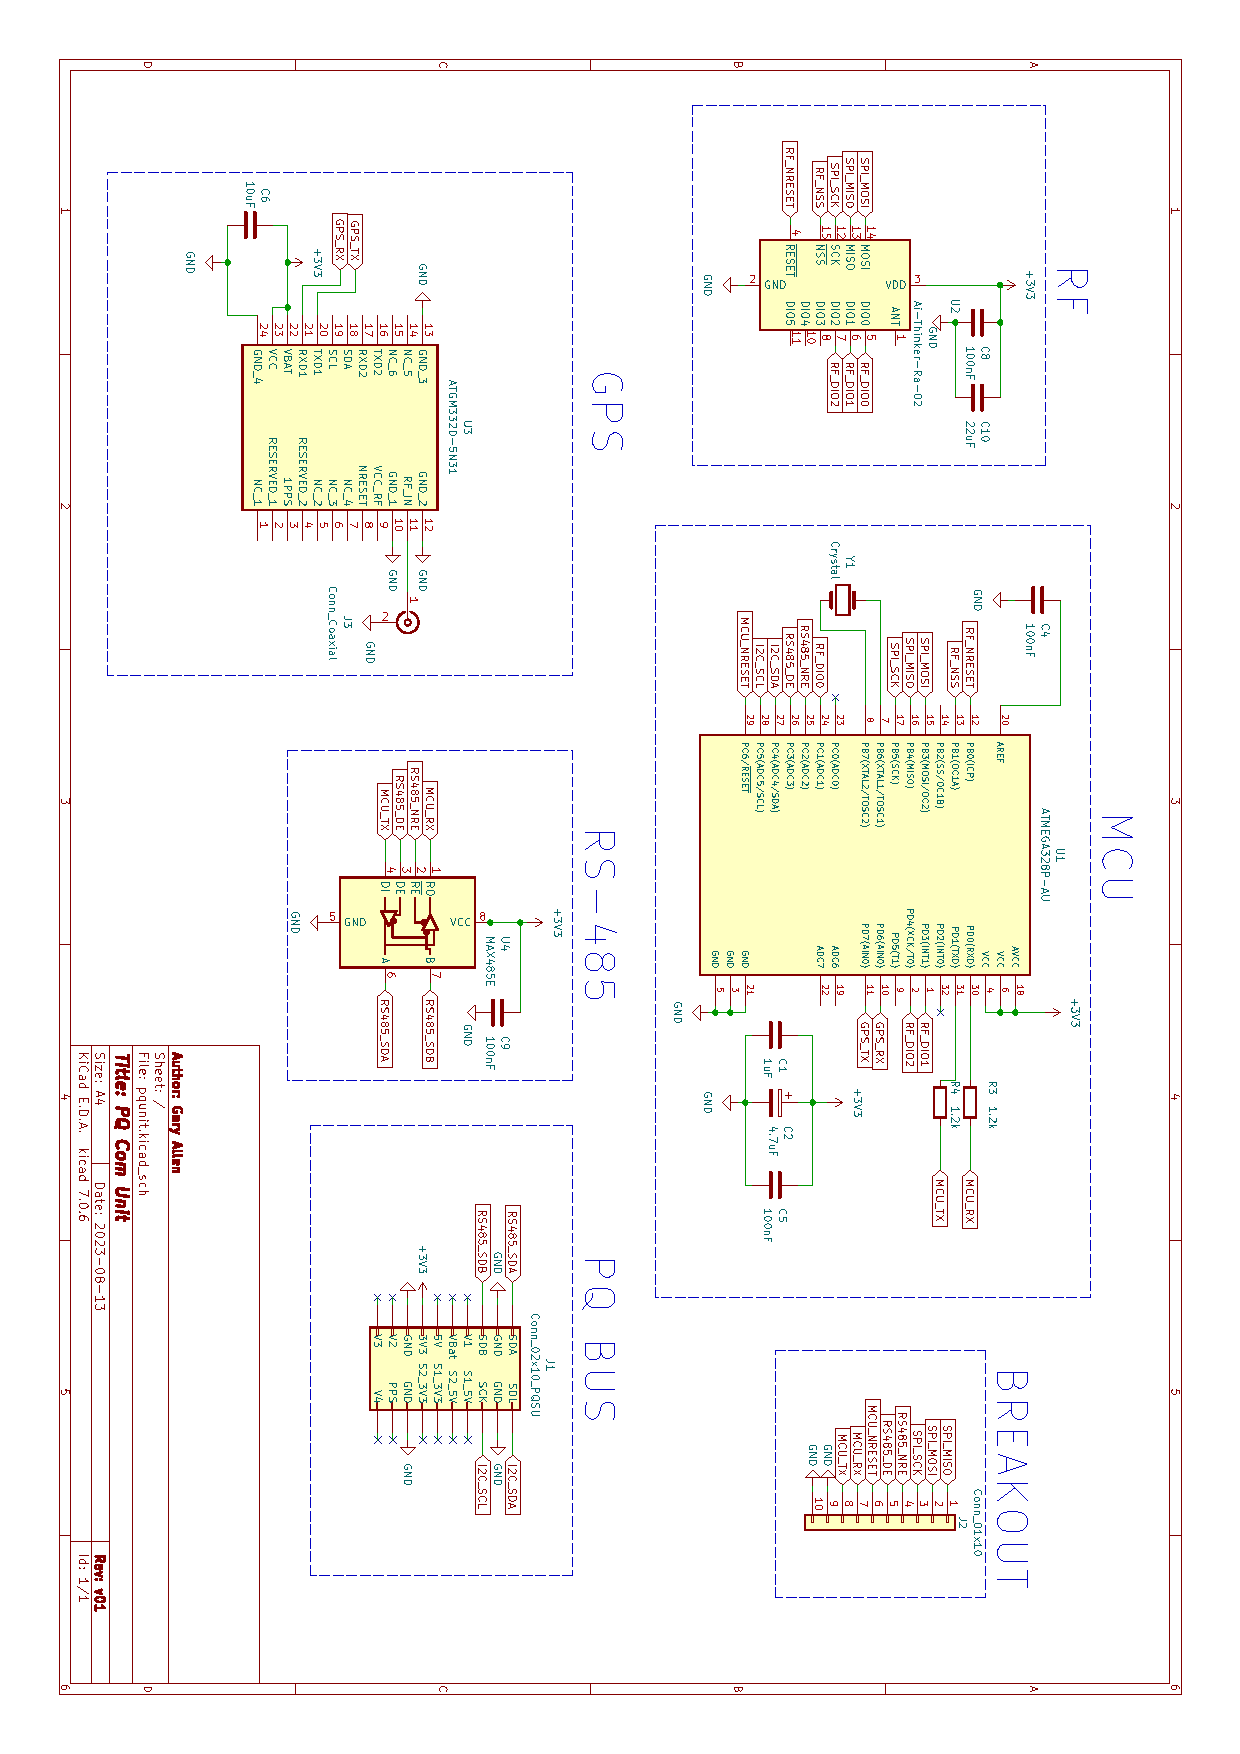
\includepdf[scale=0.65,pages=1,pagecommand=\chapter{Appendix C}\label{sec:appendix_pq_schematic}]{pq_schematic}

\end{document}